
\documentclass[conference]{IEEEtran}


\usepackage{cite}
\usepackage{color}
\usepackage{courier}
\usepackage{tikz}
\usepackage{balance} % Add this back in. Probably needed during camera ready.
\usepackage{pgfplots}
\usepackage{graphicx}% http://ctan.org/pkg/graphicx
\usepackage{listings}
\usepackage{times}
\usepackage{booktabs}
\usepackage{fancybox}

\usepackage{multirow}
\usepackage{array}
\usepackage{tabularx}
\usepackage{url}
\urlstyle{same}
\usepackage{xcolor}
\usepackage{caption}
\usetikzlibrary{shapes,arrows}
\usetikzlibrary{patterns}
\usepackage[numbers]{natbib} % Used to fix formatting issue.
\usepackage{soul} % Needed for wrapping of highlighted text

%Needed?
%\usepackage{bm}


% Define bar chart colors
\definecolor{bblue}{HTML}{4F81BD}
\definecolor{rred}{HTML}{C0504D}
\definecolor{ggreen}{HTML}{9BBB59}
\definecolor{ggrey}{HTML}{707070}
%\definecolor{ppurple}{HTML}{9F4C7C}

% Define flow chart styles
\tikzstyle{decision} = [diamond, draw, fill=blue!20,
    text width=15em, text badly centered, node distance=3cm, inner sep=0pt]
\tikzstyle{block} = [rectangle, draw, fill=blue!20,
    text width=15em, text centered, rounded corners, minimum height=4em]
\tikzstyle{line} = [draw, -latex']

\usetikzlibrary{shapes,arrows, positioning} % Needed for analysis diagram

\newcommand{\todo}[1]{\textcolor{cyan}{\textbf{[#1]}}}
\newcommand{\dan}[1]{\textcolor{blue}{{\it [Dan says: #1]}}}
\newcommand{\andy}[1]{\textcolor{yellow}{{\it [Andy says: #1]}}}
\newcommand{\sam}[1]{\textcolor{green}{{\it [Sam says: #1]}}}
\newcommand{\Mehdi}[1]{\textcolor{red}{{\it [Mehdi says: #1]}}}



\begin{document}
%
% paper title
% can use linebreaks \\ within to get better formatting as desired
\title{Maturity and Security: Static Analysis of Reverse-Engineered Android Applications}

\author{\IEEEauthorblockN{Daniel E. Krutz, Mehdi Mirakhorli, Casey Klimkowsky, Andrew Meneely,  and Samuel Malachowsky}
\IEEEauthorblockA{
Rochester Institute of Technology,
Rochester, NY, USA\\
\{dxkvse,  mxmvse,  cek3403, axmvse, samvse\}@rit.edu}
}




% use for special paper notices
%\IEEEspecialpapernotice{(Invited Paper)}




% make the title area
\maketitle


\begin{abstract}
%\boldmath

Android is currently the most popular mobile operating system in the world, with a myriad of applications (``apps'') freely available to users. As with most software, Android apps can put users at risk with inadvertent defects, vulnerabilities, and even intentionally placed malware. App stores typically mitigate these risks by moderating app reviews and managing the deployment of new releases. As a result, Android users may arrive at the belief that by upgrading their apps, they are installing a more stable and secure product. In this research, we investigate the maturity of these applications and their relationship with quality and security by statically analyzing Android applications. We collected and reverse-engineered 30,020 Android applications from the GooglePlay store and analyzed each app using six static analysis tools. We examined maturity (via release number), application size, rate of potential defects, adherence to coding standards, rate of overprivileged settings, privileges used, potential vulnerability level, and number of code clones. We also compared measurements between benign and known malware applications. Among our results were the conclusion that Android applications degrade over time in potential vulnerabilities and number of overprivileged permission settings. We have publicly released our result set for examination with a robust web-based tool.

\todo{update to include FDroid}

\end{abstract}

% no keywords




% For peer review papers, you can put extra information on the cover
% page as needed:
% \ifCLASSOPTIONpeerreview
% \begin{center} \bfseries EDICS Category: 3-BBND \end{center}
% \fi
%
% For peerreview papers, this IEEEtran command inserts a page break and
% creates the second title. It will be ignored for other modes.
\IEEEpeerreviewmaketitle


\section{Introduction}

% Get market share information from FlowDroid paper


% Use stats from http://www.androlib.com/appstats.aspx
%There are over 1,300,000 Android applications~(\emph{apps}) with thousands of new applications being created every month~\cite{appbrain_stats_url}.

Android users download more than 1.5 billion applications~(``apps'') from GooglePlay every month~\cite{androidpopularity_url}. Apps are a major part of mobile consumer technology and have changed the computing experience of our modern digital society, allowing users to perform a variety of tasks not previously possible in a portable environment.

Software, mobile or not, is in need of constant maintenance. Android apps often contain inadvertant defects and vulnerabilities that can seriously impact a mobile user. Even worse, malicious developers regularly create malware apps to attack trusting Android users. App stores such as GooglePlay mitigate these risks by managing the delivery of app updates and moderating review systems so that users can make safe choices in what they install on their devices.  As a result, apps are routinely updated for bug fixes, vulnerability mitigations, support for new hardware, and feature additions.

With a constant stream of updates, however, users may develop the perception that their favorite apps are improving as the app is maturing. Between releases, developers have the opportunity to refactor, redesign, respond to reviews, and improve the product overall. However, as an app gains users, the size and complexity of the code base can also become unwieldy, leading to a regression of quality and security.

For developers, static analysis tools are one way of identifying potential risks of defects or vulnerabilities. Modern static analysis tools have been adapted to specific platforms, such as Android, to examine risks in areas such as overprivileges, coding standards, and potential defects. In recent academic studies~\cite{Felt:2011:APD:2046707.2046779,Vidas11curbingandroid,Lee_2013}, static analysis tools have also been used as one method of measuring the quality and security of mobile software. An empirical analysis of a large body of Android applications over time can therefore provide a broad view into what ``improvements'' users are seeing as their apps are continually updated.

\emph{The goal of this work is to provide a overall understanding of the relationship between the maturity of mobile applications with potential quality and security defects.} We collected and reverse engineered 30,020 Android applications in 41 different genres from the GooglePlay store. We analyzed each of the apps using six static analysis tools: Stowaway~\cite{Felt:2011:APD:2046707.2046779}, AndroRisk~\cite{androguard_url}, CheckStyle~\cite{checkstyle_key}, JLint~\cite{jlint_key}, Simcad~\cite{6613857}, and APKParser~\cite{apkparser_link}.  We examined maturity (via the release number), application size, rate of potential defects, adherence to coding standards, rate of overprivileged settings, potential vulnerability level, and number of code clones. We also compared our measurements between benign and known malware applications. Finally, we examined the relationship between our quality metrics and security metrics.

The contributions of this work are:

\begin{itemize}
  \item An empirical analysis of how potential defects and vulnerabilities evolve over time in Android applications.
  \item A public data set of our results for future analysis by other researchers. This includes robust search and reporting mechanisms.
\end{itemize}

\section {Research Questions}
\todo{update all of these with the new questions}
This research is guided by the following questions. More details on how we collected our data can be found in Section~\ref{sec: collection}, and details on how we analyzed these metrics can be found in Section~\ref{sec: analysis}.

\textbf{RQ1:}~\emph{Does the number of potential security risks increase over time?}\\
We explore if applications increase or decrease in their potential security risks. The security risks we examine are overprivileges and identification of vulnerabilities as identified by a static analysis tool. This analysis is discussed in Section~\ref{sec: evaluation}.

We perform this analysis with Stowaway to measure overprivileges and Androrisk to measure an application's risk. See section~\ref{sec: analysis} for more details on these metrics.


\textbf{RQ2:}~\emph{What are the most pervasive overprivileges?}\\
Defining overly broad permissions for an Android app is a simple mistake that can lead to security issues arising in the future. We measured the number and types of overprivileges across our data set to examine the most common mistakes.

\textbf{RQ3:}~\emph{What is the variation of risks across genres?}\\
Different types of apps may lend themselves to different kinds of maturity, feature evolution, or security risks. We evaluate our results within GooglePlay genres.

\textbf{RQ4:}~\emph{Are benign apps measured as more secure when compared against known malware?}\\
To investigate the soundness of the static analysis tools and our measurements, we compare our measurements against a population of known malware. We examine the same risks as we did in RQ1.


\section{Related Work}
\label{sec: relatedwork}

% \todo{This section needs to be changed to not just address the permissions gap}
% \todo{make sure this section is really good, I can see people really scrutinized this.}

Android applications have been extensively researched in numerous areas. The topic of reducing the permission gap in Android applications has received a considerable amount of attention recent years. Much of the existing work in this area has dealt with ways of reducing these unneeded permissions and the security vulnerabilities they may lead to. Jeon~\emph{et al.} introduced a framework for creating finer-grained permissions in Android. They believe that the course-grained permissions currently used by Android limit developers by forcing them to choose all of the permissions located in each ``bucket'' when they really only want to add a few of them. This leads to applications having many more permissions than they actually require. The authors believe that finer-grained permissions would lead to only having the needed permissions used by an application, and thus would lead to few vulnerability possibilities~\cite{jeon2011dr}.

Wei~\emph{et al.} studied the evolution of Android to determine if the platform was allowing the system become more secure. They found that the privacy and security in the overall Android system is not improving over time and that the principle of least privilege is not being adequately addressed~\cite{Wei:2012:PEA:2420950.2420956}.

There have been innumerable studies analyzing mobile applications on a large scale. Sarma~\emph{et al.} evaluated several large datasets, including one with 158,062 Android applications in order to gauge the risk of installing the application, with some of the results broken down by genre. However, this work did not analyze the application using the range of static analysis tools which we used. Viennot~\emph{et al.} developed a tool called PlayDrode which they used to examine the source code of over 1,100,000 free Android applications. While the authors examined a very large number of applications, they largely only used existing information which could be gathered from GooglePlay and, while they carried out static analysis on the applications, they examined features such as library usage and duplicated code --- not areas such as security vulnerability levels and overpriviledges, which was a part of our analysis.


While this work represents the largest known empirical analysis of developers allowing overprivileges to occur in Android applications, it is not the first research into developers not following the principle of least privilege. Felt~\emph{et al.} described some common developer errors found using their tool Stowaway including confusing permission names, the use of depreciated permissions, and errors due to copying and pasting existing code~\cite{Felt:2011:APD:2046707.2046779}. In another work, Felt~\emph{et al.} very briefly described some inclinations they had for why developers gave too many permissions to applications, but this was largely based on assumptions and not necessarily data~\cite{Felt:2011:EAP:2002168.2002175}.


%There have been several tools which have been developed to assist in the decision making, permission process for developers. Felt~\emph{et al.} created a tool known as~\emph{Stowaway} which uses a permissions-to-API calls maps in order to statically analyze request permissions in Android applications~\cite{Felt:2011:APD:2046707.2046779}. This tool notes the extra, unneeded permissions requested by the application, along with permissions that should have been requested, but were not. One criticism of this tool is that it may be difficult to determine if a permission is actually used through the use of static analysis.

Permlyzer is a tool which was built to determine where permissions are utilized in Android applications by using a mixture of static and runtime analysis~\cite{6698893}. This is a recently published tool, so it has not yet been discussed or used in a substantial amount of subsequent research. The authors were, however, able to achieve promising results and this may be a powerful tool for assisting in the permissions granting decision process for developers. \emph{PScout} was another tool developed to extract permission specifications from Android applications using static analysis~\cite{Au:2012:PAA:2382196.2382222}. While the authors of this tool were able to achieve promising results, subsequent work has criticized this tool for not being accurate enough, since Android's permissions could be different at runtime --- something the tool is not capable of discovering~\cite{zhang2013vetting}.

Bartel~\emph{et al.} and Wei~\emph{et al.} also discussed some basic, high level discoveries about why developers make these mistakes~\cite{Bartel:2012:ASP:2351676.2351722,Wei:2012:PEA:2420950.2420956}. While these works were beneficial for numerous reasons, no known works to date have explored the question of why developers do not adhere to the principle of least security as consistently as they should.


%%% Based on ICSE Feedback, add information from related work
% Ryan Stevens, Jonathan Ganz, Vladimir Filkov, Premkumar T. Devanbu, Hao Chen:
% Asking for (and about) permissions used by Android apps.MSR 2013: 31-40




\label{sec: androidapplications}
\section{Android Applications}


The Android operating system is the most popular mobile platform in the world with apps being available on numerous types of devices from a variety of manufacturers~\cite{androidpopularity_url}. This flexibly has allowed the Android operating system to flourish, but results in many different hardware platforms and OS versions for app developers to support.

\subsection{Android Application Structure}

The Android application stack is comprised of four primary layers. The top layer is the Android application layer, which is followed by the the three application framework layers. The Android Software Development Kit (SDK) allows developers to create Android applications using the Java programming language. Isolation between Android applications is enforced through the use of the Android sandbox~\cite{androidsecuritytips_url}, which typically prevents applications from intruding upon one another.

%% This section is probably no longer needed - DK 1/14/15
%\emph{Intents} are a communication mechanism to exchange information between the components (\emph{Activities}) of an Android application, and are reported to the user upon installation and use. Inter Process Communication (IPC) is the composition mechanism performed using Intents which is used to invoke another application component. Attacks that exploit Intents for malicious reasons include ~\emph{permission collusion},~\emph{confused deputy}, and~\emph{intent spoofing}~\cite{Chin:2011:AIC:1999995.2000018,grace2012systematic, Marforio:2012:ACC:2420950.2420958, 6641043}.

Android applications are packaged in APK files, which are compressed application files which includes the application's binaries and package metadata. Table~\ref{Table:apkcontents} shows the breakdown of a typical APK file.

%% Much of this able came from : ~\cite{Lee_2013}
\begin{table}[ht]% Try here, and then top
\begin{center}
\caption{APK Contents}
\label{Table:apkcontents}
  \begin{tabular}{| l | l | } \hline

    \bfseries File & \bfseries Description \\ \hline
    AndroidManifest.xml & Permissions \& app information \\ \hline
    Classes.dex & Binary Execution File \\ \hline
    /res & Directory of resource files \\ \hline
    /lib & Directory of compiled code \\ \hline
    /META-INF & Application Certification \\ \hline
    resources.arsc & Compiled resource file \\ \hline
  \end{tabular}
  \end{center}
\end{table}


Android applications are available from a variety of different locations including AppksAPK\footnote{http://www.appsapk.com/}, F-Droid\footnote{https://f-droid.org/}, and the GooglePlay store\footnote{https://play.google.com/store}. These variety of offerings differ from the iOS app store, which forces all non-jailbroken devices to access applications through an Apple controlled store. GooglePlay provides verification of uploaded applications using a service called Bouncer which scans applications for malware~\cite{bouncer_url1}. In spite of these efforts, malicious apps are sometimes found on the GooglePlay store~\cite{Zhou:2012:DAM:2310656.2310710}. GooglePlay separates apps into~\emph{Genres} based on their realm of functionality, some of which are Action, Business, Entertainment, Productivity, and Tools. The~\emph{AndroidManifest.xml} file contains permissions and application information as defined by the developer.



\subsection{Android Permission Structure}
Android developers operate under a permission-based system where apps must be granted access to various areas of functionality before they may be used. If an app attempts to perform an operation which it does not have permission, a~\emph{SecurityException} is thrown. When an Android app is created, developers must explicitly declare in advance which permissions the application will require~\cite{Felt:2011:APD:2046707.2046779}, such as the ability to write to the calendar, send SMS messages, or access the GPS.

When installing the application, the user is asked to accept or reject these requested permissions. Once installed, the developer cannot remotely modify the permissions without releasing a new version of the application for installation~\cite{shaerpour2013trends}, prompting the user if new permissions are required. These security settings are stored in the AndroidManifest.xml file and include a wide range of permissions, some of which are~\emph{INTERNET},~\emph{READ\_CONTACTS}, and~\emph{WRITE\_SETTINGS}. Unfortunately, developers often request more permissions than they actually need, as there is no built in verification system to ensure that they are only requesting the permissions their application actually uses~\cite{Felt:2011:APD:2046707.2046779}.

A basic principle of software security is the~\emph{principle of least privilege}, or the granting of the minimum number of privileges that an application needs to properly function~\cite{saltzer1975protection}. Granting more privileges than the application needs creates security problems since vulnerabilities in other applications, or malware, could use these extra permissions for malicious reasons. Additionally, this limits potential issues due to non-malicious developer errors. Unfortunately, due to the lack of granularity of the permission spectrum used by Android, the developer must often grant more permissions to their application than it actually requires. For example, an application that needs to send information to one site on the internet will need to be given full permissions to the internet, meaning that it may communicate with with all websites~\cite{jeon2011dr}.

In this paper, we use the term \emph{overprivilege} to describe a permission setting that grants more than what a developer needs for the task. Likewise, an \emph{underprivilege} is a setting for which the app could fail because it was not given the proper permissions. Overprivileges are considered security risks, underprivileges are considered quality risks.




\label{sec: dca}
\section{App Collection \& Static Analysis}
\todo{update entire section}
We analyzed 30,020 Android application files over a period of 3 months using a variety of different tools. The results of this analysis have been stored in a publicly accessible database located on our project website\footnote{http://darwin.rit.edu}. Our methodology is as follows:

\begin{enumerate}
  \item Collect APK files
  \item Reverse-engineer binaries
  \item Execute static analysis tools
  \item Complete evaluation (see Section~\ref{sec: evaluation})
\end{enumerate}

We created the~\emph{Darwin} tool that downloads Android Application (.apk) files and invokes various static analysis tools against these files.

\label{sec: collection}
\subsection{Step 1: Collect APK files}
\todo{update for F-Droid}

Android APK files were pulled from GooglePlay with a custom-built collector, which used~\emph{Scrapy}~\footnote{http://scrapy.org} as a foundation. We chose to pull from GooglePlay since it is the most popular source of Android applications~\cite{listofstores_URL} and was able to provide various application information such as the developer, version, genre, user rating, and number of downloads. To limit the impact of seldom-downloaded applications, we divided of our results into two groups: applications with at least 10,000 downloads, and those with less than 10,000 downloads. Of the 30,020 applications downloaded, 12,215 had at lt least 10,000 downloads, while 17,805 had fewer.

%To limit the impact of seldom-downloaded applications, we only included applications with at least 10,000 downloads in our results. Of the 30,020 applications downloaded, 12,215 had at lt least 10,000 downloads, while 17,805 had fewer. In our presented results, unless otherwise noted the data set we will be referencing is the one comprising applications with at least 10,000 downloads. \dan{I added above...State why?}

\subsection{Step 2: Reverse-engineer binaries}
\label{sec: decompliation}

Some of our static analysis tools require source code instead of binary code, so we followed a reverse engineering process similar to that as proposed by previous research~\cite{Lee_2013,6687155}. For many of our static analysis tools, the downloaded APK files had to be decompiled to .java files. The first step was to unzip the .apk file using a simple unix command, which creates the files shown in Table~\ref{Table:apkcontents}. Next, we used two open source tools to complete the reverse engineering process. These were:

\begin{itemize}
  \item \textbf{dex2jar~\cite{dex2jar_key}:} Convert the .dex file into a .jar file. A java jar command is then used to convert this to .class files.
  \item \textbf{jd-cmd~\cite{jdcmd_key}:} A command line decompiler that converts .class files to .java.
\end{itemize}

Additionally, we recorded the number of extracted class and java files. The de-compilation process is shown in Figure~\ref{fig:extractionprocess}.



% ~\cite{Lee_2013} %% This diagram is largely copied from here

% Define block styles
\tikzstyle{line} = [draw, -latex']
\tikzstyle{cloud} = [draw, ellipse,fill=white!20, node distance=2.2cm,
    minimum height=2em]

	\begin{figure}[h]
	\begin{center}
\label{fig:extractionprocess}
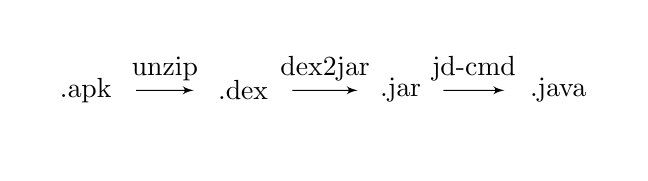
\begin{tikzpicture}[node distance = 2cm, auto]
    % Place nodes
     \node [cloud] (init) {.apk};
     \node [cloud, right of=init] (dex) {.dex};
     \node [cloud, right of=dex] (jar) {.jar};
     \node [cloud, right of=jar] (java) {.java};

     \path [line] (init) -- node {unzip}(dex);
     \path [line] (dex) -- node {dex2jar}(jar);
     \path [line] (jar) -- node {jd-cmd}(java);

\end{tikzpicture}
\caption{APK Extraction Process}
\end{center}
\end{figure}


\subsection{Step 3. Execute static analysis tools}
\label{sec: analysis}

\todo{update to include only the used tools}

The next phase was to analyze the extracted source code for a variety of metrics, including potential security risks, permissions issues, potential non-security defects, and misuse of coding standards. We also collected information about software clones, which are functionally equivalent portions of an application that may differ syntactically. A sign of poorly written software, clones may be detrimental to an application in a variety of ways, including increased maintenance costs and inconsistent bug fixes~\cite{Roy:2009:CEC:1530898.1531101}. We used the following tools for our analysis:

 \textbf{Stowaway\cite{Felt:2011:APD:2046707.2046779}:} Reports the overprivileges and underpriviledges of an application, which we recorded. Slight modifications were made to the existing version of Stowaway to accommodate our process and current Android applications with updated permissions. Permlyzer~\cite{6698893}, a more modern permission detection tool, was not used since its authors have not made it available for download.

 \textbf{AndroRisk\cite{androguard_url}:} A component of the Androguard reverse engineering tool which reports the risk indicator of an application for potential malware. We recorded the reported risk level for each APK file. \todo{Add more analysis of Androrisk and how it calculates the risk level}

%%% ? Mention that Sonar was only ran on F-Droid apps since we had many versions of these apps?
 \textbf{Sonar:} Blah \todo{update this}
% Good definitions http://docs.sonarqube.org/display/SONAR/Metric+definitions

\footnote{\url{http://docs.sonarqube.org/display/SONAR/Metric+definitions}}

Stowaway and Androrisk were able to analyze the raw APK files, while CheckStyle, Jlint, and Nicad required the APK files to be decompiled. All results were recorded in an SQLite~\footnote{http://www.sqlite.org/} database, which is publicly available on the project website. The full analysis process is shown in Figure~\ref{fig:analysisprocess}.

\begin{figure}[h]
\begin{center}
\label{fig:analysisprocess}
% Define block styles
\tikzstyle{line} = [draw, -latex']

%\tikzstyle{cloud} = [draw, ellipse,fill=white!20, node distance=1.5cm, minimum height=2em]
\tikzstyle{cloud} = [draw=none, ellipse,fill=white!20, node distance=1.5cm, minimum height=2em]

\tikzstyle{block} = [rectangle, draw, fill=white!20, text width=5em, text centered, rounded corners, minimum height=4em]
\tikzstyle{c} = [draw, cylinder, shape border rotate=90, aspect=0.75, minimum height=70, minimum width=30]

\begin{tikzpicture}[node distance = 1.5cm, auto]

    % Place nodes
     \node [cloud] (init) {APK Collection};
     \node [block, below of=init] (ApkFiles) {ApkFiles};
     \node [cloud, below of=ApkFiles] (Decompile) {Decompile};
     \node [block, below of=Decompile] (DecompiledFiles) {Decompiled Files};
     \node [cloud, below of=DecompiledFiles] (JavaAnalysis) {Java Analysis};
    % \node [cloud, right of=ApkFiles] (apkanalysis) {Stowaway AndroRisk};
    % \node [c, right of=DecompiledFiles] (SqliteDB) {SqliteDB};
     \node[c] (SqliteDB) [below right=-1.0cm and 2.4cm of DecompiledFiles]{SQLiteDB};

    \node[cloud] (apkanalysis) [below right=-0.9cm and 2.0cm of ApkFiles]
       {APK Analysis};

    % Draw edges
    \path [line] (init) -- (ApkFiles);
    \path [line] (ApkFiles) -- (Decompile);
    \path [line] (Decompile) -- (DecompiledFiles);
    \path [line] (DecompiledFiles) -- (JavaAnalysis);
    \path [line] (ApkFiles) -- (apkanalysis);
    \path [line] (apkanalysis) -- (SqliteDB);
    \path [line] (JavaAnalysis) -- (SqliteDB);
    \path [line] (Decompile) -- (SqliteDB);

\end{tikzpicture}
\caption{APK Analysis Process}
\end{center}
\end{figure}

\todo{Is analysis process needed}


\section{Evaluation}
\label{sec: evaluation}


We evaluated the reverse-engineered Android applications in a variety of ways including comparing the effects of the maturity level, comparing benign applications to malware, and comparing genres with one another.


\todo{Make sure to define the violation levels from Sonar in the tools section}
\subsection{RQ1: How do Android Apps Evolve over time?}

% State what were are trying to do
% How was it done
% What are the results
% Dig deeper into this


We examined how Android applications evolved over time in terms of security risk level, over \& under privileges, and against a variety of static analysis metrics from Sonar. From our F-Droid pool of apps, we found 392 that had 3 defined versions which we had analyzed using our static analysis tools. We then broke the results into three aggregate groups of the first, second and third versions of the app and calculated the average values for each group. The results are shown in Figure~\ref{fig:VersionEffect}.


-- In order to better display the results



upriv
opriv
nlocc
violations

\todo{Add in other metrics to this table?}
% Query 4
% Good site
% 	http://tex.stackexchange.com/questions/134346/different-marker-shape-for-pgf-tikz
\begin{figure*}
\begin{center}
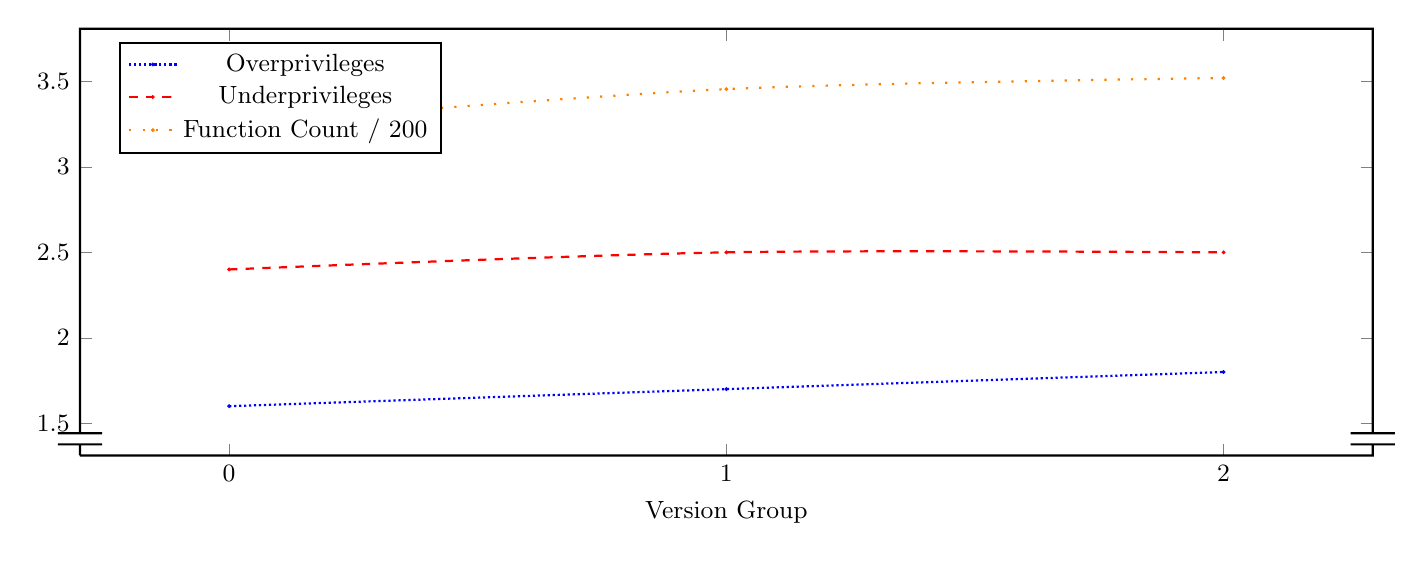
\begin{tikzpicture}
\begin{axis}[
   smooth,
   width=18cm,
   height=7cm,
   enlargelimits=0.15,
  xlabel={Version Group},
  xtick=data,
  x tick label style={rotate=0,anchor=north},
% legend pos=north west, % original
  legend pos=north west, font=\small, ,line width=.8pt,mark size=.2pt,
 axis y discontinuity=parallel,
]

% Defects - Jlint
%\addplot [color=green,dotted,mark=*,mark options={solid},smooth] plot coordinates {(0,4.9) (1,5.6) (2,6.0) (3,6.3) (4,6.4) (5,6.7)};
%\addlegendentry{AndroRiskRisk}
%\addplot [color=black,densely dotted,mark=*,mark options={solid},smooth] plot coordinates {(0,3.8) (1,4.2) (2,3.7) (3,3.7) (4,3.6) (5,3.2)};
%\addlegendentry{Jlint}
%\addplot [color=blue,dashdotted,mark=*,mark options={solid},smooth] plot coordinates {(0,2.56) (1,2.44) (2,2.9) (3,3.79) (4,3.9) (5,4.2)};



\addlegendentry{Overprivileges}
\addplot [color=blue,densely dotted,mark=*,mark options={solid},smooth] plot coordinates {(0,1.6) (1,1.7) (2,1.8)};

\addlegendentry{Underprivileges}
\addplot [color=red,dashed,mark=*,mark options={solid},smooth] plot coordinates {(0,2.4) (1,2.5) (2,2.5)};

\addlegendentry{Function Count / 200}
\addplot [color=orange,loosely dotted,mark=*,mark options={solid},smooth] plot coordinates {(0,3.25) (1,3.455) (2,3.52)};



%\addlegendentry{Clones / 100}
%\addplot [color=red,dashed,mark=*,mark options={solid},smooth] plot coordinates {(0,.1) (1,.7) (2,.6) (3,.4) (4,.1) (5,.1)};
%\addlegendentry{Coding Standards}

% Divided by 1000 to normalize
% \addplot [color=black,solid,mark=*,mark options={solid},smooth] plot coordinates {(0,6.66) (1,9.09) (2,12.87) (3,16.43) (4,18.19) (5,18.97)};
% \addlegendentry{ClassFiles / 100}
% Ratings
%\addplot [color=red,dashed,mark=*,mark options={solid},smooth] plot coordinates {(0,2) (1,2) (2,4.2) (2,3) (3,8) (4,7)(5,7)(6,1)};
%\addlegendentry{Ratings}
% Security Risk
% Values divided by 10 to normalize

%\addplot+[mark=none, draw=black] coordinates {(2,20) (2010-1,40)};
%\addlegendentry{Project Change}
\end{axis}
\end{tikzpicture}
\label{fig:VersionEffect}
\caption{Maturity and Metrics (RQ1)}
\end{center}
\end{figure*}


Across the three versions of the apps, we found that the Androrisk, over \& under privilege ratios, and other violations did not significantly vary while the number of lines of code and function count expectedly grew. This indicates that possible security issues are typically introduced in the first version of an application, and are not increased or removed throughout the life cycle of an application. 



We next  examined why privilege issues exist in applications by examining the version control histories for each app. 
Do projects where developers comment about permission/privilege issues have less of a privilege issues? In order to answer this, we will compare the average over \& under privilege ratio for apps where developers make comments about privileges compared to projects where developers make no comments about permission/privileges.


We first compared the ratio of comments pertaining to permission keywords such as the word "permission" or about the names of any of the XXX Android permissions appeared as a comment in the version control commit history to apps which had at least one overpriviledge. These results are shown in Table~\ref{table:commentratio}.

-	State exactly how we did this



%% Query 5 builds excel sheet CommentCorrelations.xlsx
\begin{table}[t]
\begin{center}
\caption{Comment Ratio}
\label{table:commentratio}
  \begin{tabular}{ | l | c | c | c | c |} \hline

 %\bfseries App  Contains OverPriv& \bfseries \%Having Comment & \bfseries Comment Ratio \\ \hline
% Yes & x & x  \\ \hline
%   No & x & x  \\ \hline

 \bfseries App  Contains OverPriv& \bfseries OverPriv & \bfseries UnderPriv \\ \hline
 All apps & .53 & 1.35  \\ \hline
 With Comments & 1.06 & 2.16  \\ \hline

  
  \end{tabular}
  \end{center}
\end{table}

\todo{should these values be correlated with size/number of commits?}
\todo{Add more things like permission names to search criteria}

%	Opriv	Upriv
%Total	0.53	1.35
%Total With commitCount >0	1.06	2.16



We then examined the the version control histories at a more individual level % breaking apps into the categories 



%In order to better understand why this occurs, we examined the repositories of several F-Droid applications looking at several situations.



 \textbf{Situation 1} 


%%%% No problems


32 - 0,0
- 2 comment about modifying permissions
- 1 author


578 0,0
- A few main authors
- 3 comments about permissions


680 0,0
- 1 comment about permissions 
- 3 main authors


855 0,0
- 1 primary author
- no comments about permissions or security

862 0,0
- 1 primary author
- no comments about permissions or security

874 0,0
- 1 primary author
- no comments about permissions or security


%%%% Problems throughout
- 23 - 3,4 - remain steady
-	1 author
-	2 comments about permissions


24 - 1,2 - steady
- 1 author
- No comments about privs or permissions


33 1,3->1,5
- 1 author
- no comments

44 1,2
- looks like there are a few authors
- no comments about priv or security


45 2,0
- 19 different authors
- 1 comment about permission


540 0,4
- 2 authors
- No comments about security


548 0,4
- No GH


612 3,0 -> 4,0
- Only a few commits. 1 author. 1 statement about permissions
- 


617 1,5 -> 1,6
- A few authors
- 1 comment about permission


653 2,2
- A few statements about permissions
- 2 more authors


684 1,2
- ~3 primary authors
- 12 comments about security and permissions


710 3,0
~6 primary authors
- 5 comments about security


711 1,1->0,3
- ~4 permissions
- Removed permission since it was not needed


724 2,3 -> 2,4
- ~6 authors
- 6 comments about permissions



735 2,0
- ~6 different authors
- 4 comments about permissions



761 2,2




766 0,4->0,2




776 0,2->1,3





778 2,6



800 2,4



823 6,3




830 8,1



902 0,6


%%%% Problems get better
%%%% Problems get worse
%%%% Interesting
18 - Opriv increases, upriv decreases
-	App all had the same author
-	Nothing interesting in the commit messages

22 - Both increase % http://sourceforge.net/p/xwords/git/ci/master/tree/xwords4/
-	Same author
-	No comments about security




-- Check to see about comments about security and rate
--		Get aggregate for both
--		Talk about overall value first and then look at these specific instances next



\subsection{RQX: What are the most  occurring over permissions?}



\subsection{RQX: What are the most  occurring over permissions?}


\subsection{RQ2: What are the most pervasive overprivileges?}


\todo{Provide analysis for all of this}
A basic principle of security is the concept of granting of the least amount of privileges to an application that it needs to properly function. Granting extra privileges creates unnecessary security vulnerabilities. Previous research has found that while Android developers try to follow this principle, they often add extra privileges to make the app work properly or, due to confusion over the permission name, they add it unnecessarily believing its functionality sounds related to their app~\cite{Felt:2011:APD:2046707.2046779}.

We analyzed the most overused permissions in 41 application genres ranging from Communication and Productivity to Sports, Puzzles, and Entertainment. We separated the applications into two groups, those with at least 10,000 downloads, and those with fewer. In Table~\ref{Table:mostoverpermissions}, we show all permissions types which had an overprivilege rate of at least 2.5\% in either group of downloads. Complete results may be found on the project website.

% # TOPOCCURINGOVERPRIVS
\begin{table}[ht]
\begin{center}
\caption{Top Occurring Overprivileges }
\label{Table:mostoverpermissions}
  \begin{tabular}{| l | c | c | } \hline

 & \multicolumn{2}{ c | }{\bfseries \ Source} \\ \hline
   \bfseries Permission  & GooglePlay  &   F-Droid \\ \hline

    ACCESS\_COARSE\_LOCATION &	x  &	x \\ \hline
    ACCESS\_FINE\_LOCATION	 & x	& x \\ \hline
    XXXX	 & XXX	& XXX \\ \hline

  \end{tabular}
\end{center}
\end{table}

\todo{update this table}


Some widely occurring overprivileges in both groups were~\emph{GET\_ACCOUNTS}, which permits access to the list of accounts in the accounts service,~\emph{READ\_EXTERNAL\_STORAGE}, which allows the application to read from an external storage device, and ~\emph{CALL\_PHONE}, which allows an application to start a phone call without the user confirming it through the dialer interface~\cite{manifest_url}. The permission~\emph{GET\_ACCOUNTS} is potentially dangerous since a malicious application could gain access to all device accounts.~\emph{READ\_EXTERNAL\_STORAGE} is potentially dangerous since an application could be granted access to information which it may not need or should not see, while~\emph{CALL\_PHONE} could allow a dangerous application to dial any phone number without the consent of the user. Previous research~\cite{Felt:2011:APD:2046707.2046779} has also found that many of our top identified overprivileges, including~\emph{ACCESS\_NETWORK\_STATE}~\emph{READ\_PHONE\_STATE}, and~\emph{WRITE\_SETTINGS} are commonly found to be unnecessary permissions.

We next examined pairs of overpriviledges which frequently occurred together in each group. In Table~\ref{Table:OverPrivsTogether}, we display all instances of permissions that occur together in at least 1.5\% of applications in either group of at least 10,000 downloads, and that of less than 10,000 downloads. One commonly occurring overprivilege combination is CALL\_PHONE and GET\_ACCOUNTS, which is dangerous since it would allow a malicious application to gather private account information and make possibly expensive calls. READ\_PHONE\_STATE and ACCESS\_WIFI\_STATE or GET\_ACCOUNTS and ACCESS\_WIFI\_STATE could potentially allow malicious software to use the open ACCESS\_WIFI\_STATE open to gather personally identifiable information~\cite{Achara:2014:SPW:2627393.2627399}.




Overall, we found that in applications with at least 10,000 downloads, 40.7\% had at least one overpermission, 25.8\% had at least 2, and 8.2\% had 4 or more. Rates were generally higher for applications with less than 10,000 downloads. These results are shown in Table~\ref{Table:appswithoverPrivs}. In 2011, previous research found that approximately 33\% of all applications were overprivileged with only about half of those containing more than one overprivilege and only 6\% requesting more than four extra permissions~\cite{Felt:2011:APD:2046707.2046779}. This indicates that the rate of overprivileged applications is growing, along with the number of extra privileges for each of these applications. Although the number of available permissions has grown in that time the difference isn't significant enough to account for the change in overprivilege (134 available permissions in 2011~\cite{Felt:2011:APD:2046707.2046779} vs. 146 in 2014~\cite{manifestpermission}).

% Query X
\begin{table}[t]
\begin{center}
\caption{Applications With Overprivileges}
\label{Table:appswithoverPrivs}
  \begin{tabular}{| c | c | c | } \hline
& \multicolumn{2}{ c | }{\bfseries \%Apps} \\ \hline
    $ \geq \mathbf{OverPrivs}$  & F-Droid  &   GooglePLay \\ \hline

        1 &	x &	x \\ \hline
        2 &	x &	x \\ \hline
        3 &	x &	x \\ \hline
        4 &	x &	x \\ \hline
        5 &	x &	x \\ \hline
        6 &	x &	x \\ \hline
        7 &	x &	x \\ \hline
        8 &	x &	x \\ \hline
        9 &	x &	x \\ \hline
        10 &	x &	x \\ \hline
        10+ &	x &	x \\ \hline


  \end{tabular}
  \end{center}
\end{table}




\subsection{RQ3: What is the variation of risks across genres?}

We next compared the various application genres to examine their rates of overprivileges, which we computed by dividing the number of overprivileges for all applications in each genre by the total number of applications in each genre. We separated the results into applications with at least 10,000 total downloads and those with less than 10,000 downloads. The results of all genres with a rate of 2.0 or higher in either download group are shown in Table~\ref{Table:topOverGenre}.

Further analysis found the top 10 genres which had at least one overprivilege. For applications with at least 10,000 downloads, we found that Communication applications had a 77\% likelihood of having at least one overprivilege, while Role Playing and Business were tied for second with an overprivilege rate of 68\%. Complete results are shown in Table~\ref{Table:topGenre}.


% OVERPRIV_GENRE_RATIO
\begin{table}[t]
\begin{center}
\caption{Top Overprivileged Ratios Per Genre}
\label{Table:topOverGenre}
  \begin{tabular}{| l | c | c | } \hline

% OverPrivilege Ratio
   %  \bfseries Genre  & \bfseries OverPrivilege Ratio \\ \hline
    & \multicolumn{2}{ c | }{\bfseries Overprivilege Ratio} \\ \hline
\bfseries Genre  & F-Droid  &   GooglePLay \\ \hline


    XXX &	xxx & xxx \\ \hline
    XXX &	xxx & xxx \\ \hline
    
  \end{tabular}
  \end{center}
\end{table}

Next, we found the percentage of applications for each genre which contained at least one overprivilege, again separating them into groups of at least 10,000 downloads and less than 10,000 downloads. In Table~\ref{Table:topGenre}, we show all genres which had at least 60\% of applications containing at least one overprivilege in either download group.

We found that the Communication, Business, and Productivity genres frequently had at least one overprivilege (Table~\ref{Table:topGenre}), but also contained a high ratio of overprivileges as well (Table~\ref{Table:topOverGenre}). The Education, Trivia, and Weather genres were least likely to contain overprivileges. Full results may be viewed on our project website.

%#AtleasthaveXoverpermisionsinEachGenre
\begin{table}[h]
\begin{center}
\caption{\% of Genres With At Least 1 Overprivilege/App}
\label{Table:topGenre}
  \begin{tabular}{ | l | c | c |  } \hline
    % \bfseries Genre  & \bfseries \% of Apps \\ \hline

 & \multicolumn{2}{ c | }{\bfseries \%Apps} \\ \hline
    \bfseries Genre  & F-Droid  &   GooglePLay \\ \hline


        XXX & XX & XX\\ \hline
        

  \end{tabular}
  \end{center}
\end{table}

% GFix table 4

%## GENRE_COMPARISIONS - The SQL Select clause needs to be changed for each group


% Over Permissions
\begin{figure*}
\begin{center}
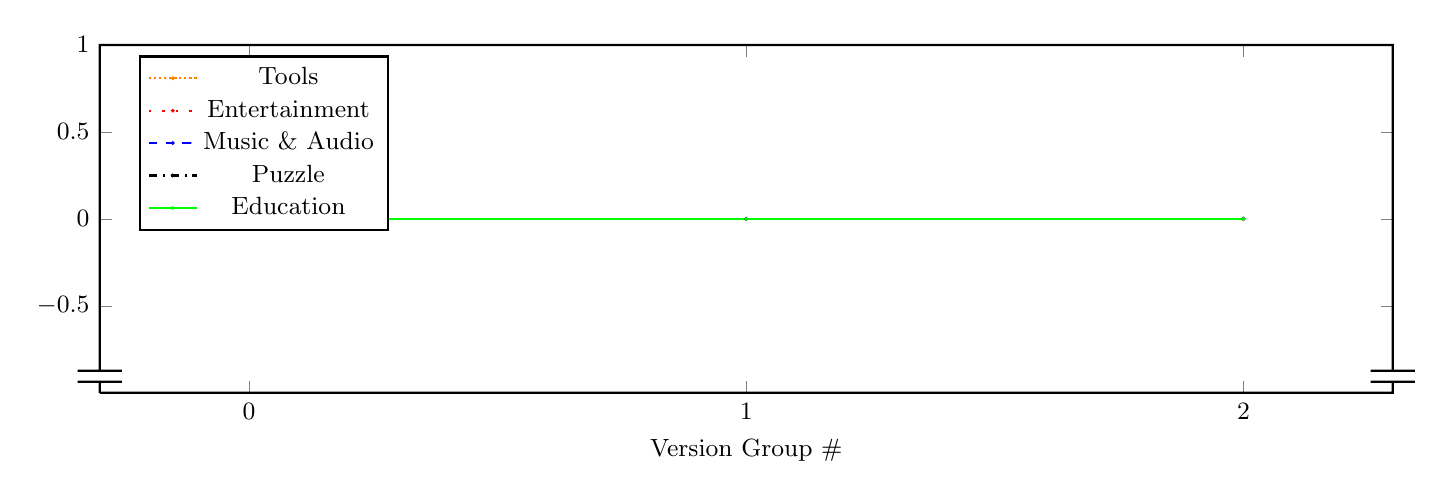
\begin{tikzpicture}
\begin{axis}[
   smooth,
   width=18cm,
   height=6cm,
   enlargelimits=0.15,
	xlabel={Version Group \#},
 %  ylabel={Values},
  symbolic x coords={0, 1, 2, 3, 4, 5},
 xtick=data,
  x tick label style={rotate=0,anchor=north},
  legend pos=north west, font=\small, ,line width=.8pt,mark size=.2pt,
 axis y discontinuity=parallel,
  ]	

\todo{Update data}


\addplot+[color=orange,densely dotted,mark=*,mark options={solid},smooth] plot coordinates {(0,0) (1,0) (2,0) };
\addlegendentry{Tools}

\addplot [color=red,loosely dotted,mark=*,mark options={solid},smooth]  plot coordinates {(0,0) (1,0) (2,0) };
\addlegendentry{Entertainment}

\addplot [color=blue,dashed,mark=*,mark options={solid},smooth] plot coordinates {(0,0) (1,0) (2,0) };
\addlegendentry{Music \& Audio}

% In this case, there were no resulst returned for puzzle for overprivs
\addplot [color=black,dashdotted,mark=*,mark options={solid},smooth] plot coordinates {(0,0) (1,0) (2,0) };
\addlegendentry{Puzzle}

\addplot [color=green,solid,mark=*,mark options={solid},smooth] plot coordinates {(0,0) (1,0) (2,0) };
\addlegendentry{Education}



\end{axis}
\end{tikzpicture}

\caption{Genres \& Overprivileges}
\label{fig:genre_oPermission}
\end{center}
\end{figure*}

%% Add in an average line to give an idea what is above and below average





Finally, we present overprivileges, AndroRisk score, and Jlint results across the top genres and version numbers as with RQ1 in Figures~\ref{fig:genre_oPermission},~\ref{fig:genre_fuzzrisk}, and~\ref{fig:genre_defect}. In each case, the top genres maintain an overall increase over time in keeping with the results of RQ1.

\subsection{RQ4: Are benign apps measured as more secure when compared against known malware?}

We compared the results of the collected applications with at least 10,000 downloads from the GooglePlay store against 139 malware examples from the Contagio Mobile Mini Dump~\cite{contagio_url} and the Malware Genome Project~\cite{Zhou:2012:DAM:2310656.2310710} for the purpose of examining the differences between malicious apps and those which were considered benign. Since many of the malware examples represented only slight alterations from their counterparts, one result from each malware family was taken from the Malware Genome Project to help limit the negative impact that families with many examples would have, creating biased results.

The compared areas included adherence to coding standards, discovered defects, permission gap, and the utilized permissions. This was accomplished by running the malicious applications through the same process as the applications collected from the GooglePlay store, described in Sections~\ref{sec: decompliation} and~\ref{sec: analysis}. The results of this analysis are available on our website and are shown in Table~\ref{Table:maliciousvsnonmalicious}.

Most Android malware is piggybacked on existing applications whose malicious code is typically loosely coupled with the host application~\cite{Zhou:2012:DAM:2310656.2310710, Deshotels:2014:DAF:2556464.2556467}. We found that malicious applications had a much higher number of coding standards mistakes per class compared to their benign counterparts while also having a slightly higher number of defects per class. While we are not able to examine the development process of malware applications and interview its developers, we are able to draw several possible conclusions. Malware developers may be less likely to care about the actual user experience as opposed to developers of reputable applications, as they are probably less worried about things such as user reviews in the long run.


Not surprisingly, the malicious applications had a much higher number of overprivileges per application ($\frac{\#overprivileges}{\# apps} $) as compared to their benign counterparts. The top 10 most commonly occurring overprivileges, their rates, and how they differ from applications collected from the GooglePlay store, are shown in Table~\ref{Table:mal_permissions}.


%The~\emph{WRITE\_EXTERNAL\_STORAGE} was the most occurring over permission an malicious applications. This permission is used to store information on an external storage device such as an SD card and is often used by malicious applications

%- Many of the other requested permissions are not surprising since they may be used to gather

% Analyze these---- Can over permissions be used by malware


\begin{table}[t]

\caption{Top Occurring Overprivileges in Malware}
\label{Table:mal_permissions}
  \begin{tabular}{ | p{5.3cm} | p{1.0cm} | p{1.2cm} | p{1.2cm} |} \hline

  \bfseries Permission&\bfseries Malware&\bfseries F-Droid  &\bfseries GooglePlay\\ \hline
  WRITE\_EXTERNAL\_STORAGE & 10.7\% & x\%  & x \%  \\ \hline
  ACCESS\_LOCATION\_EXTRA\_COMMANDS & 9.8 & x & x \\ \hline
  CALL\_PHONE& 9.8 & x & x \\ \hline
  READ\_HISTORY\_BOOKMARKS & 9.8 & x & x \ \\ \hline
  WRITE\_HISTORY\_BOOKMARKS & 8.9 & x & x \\ \hline
  READ\_SMS & 8.0 & x & x\\ \hline
  SYSTEM\_ALERT\_WINDOW & 7.1 & x & x \\ \hline
  WRITE\_SMS & 7.1 & x & x \\ \hline
  READ\_CONTACTS & 6.3 & x & x\\ \hline
  RECEIVE\_SMS & 6.3 & x & x \\ \hline
  \end{tabular}

\end{table}

% Red flags for malicious applications
% Demonstrates what malicious users like to do
% Read other papers to see what they say about permissions




\begin{table}[t]
\begin{center}
\caption{Malware vs. Non-Malicous}
\label{Table:maliciousvsnonmalicious}
  \begin{tabular}{ | l | c | c | c | c |} \hline

     \bfseries Analysis Tool  & \bfseries Malicious & \bfseries F-Droid & \bfseries GooglePlay\\ \hline
    AndroRisk & 46.25 & x & x  \\ \hline
    JLint/Class & .395 & x & x  \\ \hline
    Defect Count/Class & 11.07 & x & x  \\ \hline
    Overprivilege Ratio & 3.3 & x  & x  \\ \hline
   % Underprivilege Ratio & 1.07 & 2.4 \\ \hline
    % Intent Count & 2.05 & 2.58 \\ \hline
  \end{tabular}
  \end{center}
\end{table}


\section{Publicly Available Datasets}
\label{sec:dataset}

%% Add in information about Darwin?
\todo{Add info about F-Droid site}
Our data set is available from our publicly accessible GitHub repo\footnote{https://github.com/DroidDarwin} (linked from the Darwin website), which includes the scripts used for collecting apps and invoking the static analysis tools. The SQLite database with our complete results is updated on a regular basis from our scanning and analysis application. The goal of this dataset is to allow future researchers to both learn from and expand upon our work. This data includes the following fields for each app:

\begin{itemize}
  \item Name
  \item Version
  \item Genre
   \item Number of downloads from GooglePlay
  \item Publication date on GooglePlay
  \item GooglePlay user rating
  \item Overprivileges
  \item Underprivileges
  \item Count of Jlint reported defects
  \item Count of CheckStyle coding standards mistakes
  \item Application size
  \item Count of .java files
  \item Vulnerability risk score from AndroRisk
  \item Code clone count from Simcad
\end{itemize}

Our project website (http://darwin.rit.edu) contains information about our project, links to our GitHub repository, and a robust reporting tool which will allow users to create their own data sets from over 30,000 analyzed applications. An example screenshot of the search and reporting functionality available for individual apps is shown in Figure~\ref{fig:website1}.


\begin{figure}[ht!]
\centering
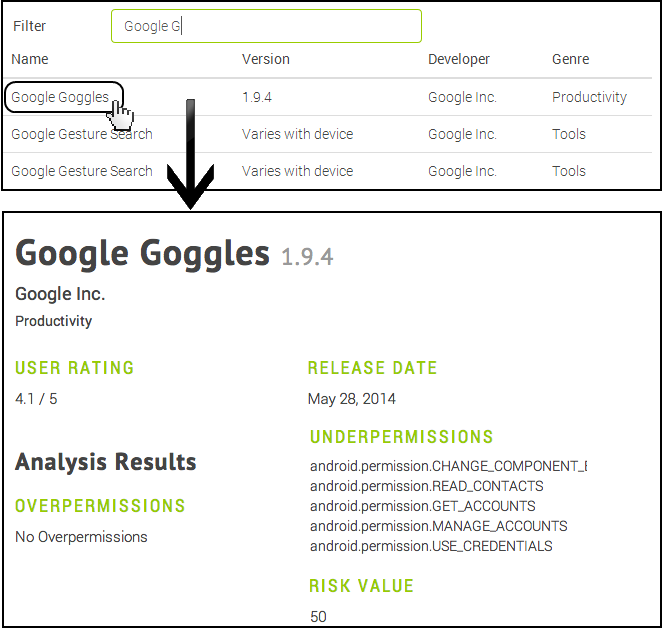
\includegraphics[width=\columnwidth, angle = 0]{images/screenshot3.png}
\caption{darwin.rit.edu Website Reporting Tool}
\label{fig:website1}
\end{figure}

\section{Limitations}
\label{sec:limitations}

While Stowaway is a powerful statical analysis tool which has been used in a substantial amount of previous research~\cite{Pearce:2012:APS:2414456.2414498,Stevens_investigatinguser,jeon2011dr}, it does suffer some drawbacks. Malicious code may be obfuscated and unnecessary API methods inserted into the application, rationalizing the permission~\cite{6698893}. Static analysis techniques can also be hindered by the Java reflection process and may lead to inaccuracies~\cite{Sridharan:2006:RCP:1133255.1134027,Tripp:2009:TET:1542476.1542486}. These types of limitations are inherent to all statical analysis tools.

We only analyzed applications from GooglePlay and F-Droid and not other sources such as AppksAPK the Google Amazon store, which would have led to more varied application origins. However, we feel the diversity of our applications was already quite robust since we collected 30,020 applications from 41 genres.\todo{update values}

We also only examined free applications in our research due to cost constants. Thus, the measurements comparison of apps is not representative of the entire Android app market. Our results only apply as a comparison of free apps, not with paid apps.

%% Add in more limitations
%   We rely on release numbers from the developer




\section{Conclusion}
\label{sec: conclusion}

%In this work, we demonstrated our technique of downloading and analyzing 30,020 Android applications in a variety of areas including security vulnerability level, overprivileges, code clones, potential defects, and coding standards mistakes. We found that, on average, Android applications increase in their potential security risks with each release while increase instances of code clones and decreasing potential defects. We conducted our analysis within genres and found that certain genres included more instances of overprivileges. As a control, we compared our analysis results against known malware and found that the static analysis tools we employed demonstrated high levels of security risk where malware was known. These results provide a broad overview of the state of the breadth of free apps in the GooglePlay store.

\balance
\bibliographystyle{abbrv}
\bibliography{AndroidData}

% that's all folks
\end{document}


%%%% Research Analysis
%   Look at version control systems to understand why everything occurs. Look at commit messages.
%


%%%% Questions
%

%%%% Todo
%   Make sure it is in MSR format
%   Add Keywords etc ??
%   Update title
%       Static Analysis of Open Source Android Applications
% Tie into the Darwin data? - Use this well and then analyze the F-Droid repos for similar information
% ? Mention Darwin
%   Make sure all the counts add up. IE the number of versions match
%   Randomly pull in 1200 apps. Say we did it X times, and it returned similar results.
%   Give user's the ability to write web queries off SQLiteDB
%   



%%% Possible actions
%     Run APKs from F-Droid on same analysis as Darwin
%	Look at the stats of apps with overprivs (sonar results) vs. apps with no violations




% RQs
%   How do apps evolve over time & what correlations exist between risk and other metrics
%   Are overprivs generally fixed?
%       Dig into some of the version control systems to determine why or why not
%   Correlation of commit comments to security & defects
%   Overprived genres & how many they have
%   If an app has one, how many other overprivs does it have?
%   Are certain overprivs added 


%%%
%	Identify potential security problems in specific apps	
%	How to actually check
%	Look at the actual permissions in the manifest file to see how the permissions change over time
%		Look into this
%	






